% Source for the figure of FlatHashTable (sec. 7.6): two groups of 15
% control bytes and a byte of overflow; the search of k, fingerprint 5A and
% overflow bit 3, matches the places 1 and 4 of g, goes past g since its
% overflow has the bit 3, and finds k in the place 2 of g + 1.
% Build: make figures (in ../build).
\documentclass[border=4pt]{standalone}
\usepackage[T1]{fontenc}
\usepackage{lmodern}
\usepackage{amsmath,amssymb}
\usepackage{tikz}
\usepackage{lamalunga}
% tikz-ads.tex: the TikZ styles shared by the figures of the memory of the
% manual, \input by each standalone figure: a cell of a vector (cell), the
% cell that an operation touches (touched), a free cell (free), a node of a
% linked structure (node), the labels of indices (index) and of variables
% (var), a pointer (ptr), and \cells and \indices to draw a row of cells.
\usetikzlibrary{arrows.meta,positioning,calc,fit,shapes.multipart}
\definecolor{adsTouched}{RGB}{214,196,236}
\definecolor{adsFree}{RGB}{236,236,236}
\tikzset{
  ads/.style={>={Stealth[length=2mm]},font=\small,
              every node/.append style={inner sep=0pt}},
  cell/.style={draw,minimum width=7mm,minimum height=7mm,
               font=\small\ttfamily,outer sep=0pt},
  touched/.style={cell,fill=adsTouched},
  free/.style={cell,fill=adsFree,text=black!45},
  node/.style={draw,rounded corners=1pt,minimum width=8mm,
               minimum height=6mm,font=\small\ttfamily},
  index/.style={font=\scriptsize\ttfamily,text=black!60},
  var/.style={font=\small\itshape},
  ptr/.style={->,thick}
}
% \cells{name}{x,y}{list}: a row of cells, the first at (x,y), named
% name-0, name-1, ...; each item is text/style, the style one of cell,
% touched and free (e.g., {a/cell,e/touched,/free})
\newcommand{\cells}[3]{%
  \foreach \v/\s [count=\i from 0] in {#3}
    \node[\s] (#1-\i) at ($(#2)+(\i*7mm,0)$) {\v};}
% \indices{name}{n}: the indices 0 .. n-1 under the cells of name
\newcommand{\indices}[2]{%
  \foreach \i in {0,...,\numexpr#2-1\relax}
    \node[index,below=1.2mm of #1-\i] {\i};}

\tikzset{cb/.style={cell,minimum width=6.5mm,minimum height=6mm,font=\scriptsize\ttfamily},
         cbt/.style={touched,minimum width=6.5mm,minimum height=6mm,font=\scriptsize\ttfamily\bfseries},
         cbf/.style={free,minimum width=6.5mm,minimum height=6mm,font=\scriptsize\ttfamily},
         ob/.style={cell,minimum width=3mm,minimum height=6mm,font=\tiny\ttfamily,line width=0.6pt},
         obt/.style={touched,minimum width=3mm,minimum height=6mm,font=\tiny\ttfamily\bfseries,line width=0.6pt}}
\newcommand{\grp}[3]{% name, y, bytes
  \foreach \v/\s [count=\i from 0] in {#3}
    \node[\s] (#1-\i) at (\i*6.9mm,#2) {\v};}
\newcommand{\ovf}[3]{% name, y, bits 7..0
  \foreach \v/\s [count=\i from 0] in {#3}
    \node[\s] (#1-\i) at (108mm+\i*3.3mm,#2) {\v};}
\begin{document}
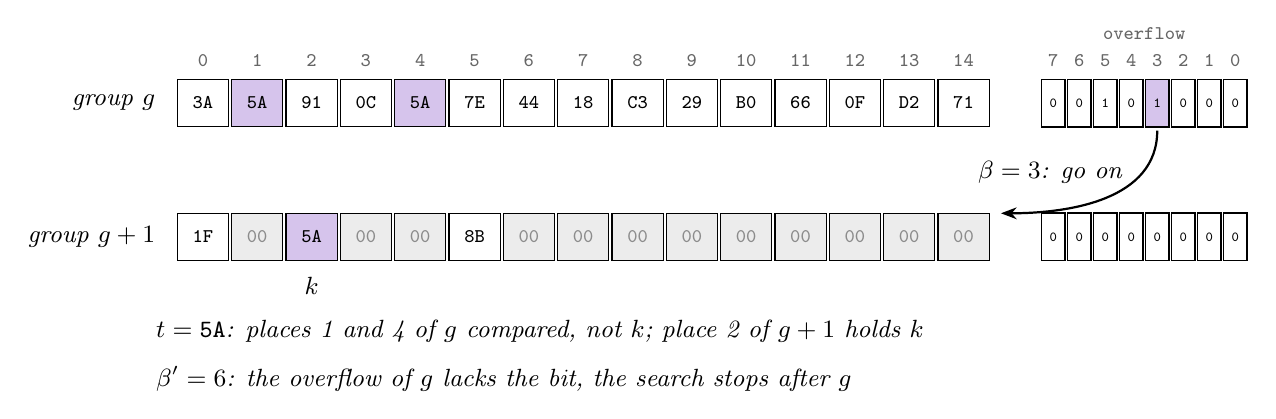
\begin{tikzpicture}[ads]
  \node[var,anchor=east] at (-6mm,0) {group $g$};
  \grp{g}{0}{3A/cb,5A/cbt,91/cb,0C/cb,5A/cbt,7E/cb,44/cb,18/cb,C3/cb,29/cb,B0/cb,66/cb,0F/cb,D2/cb,71/cb}
  \ovf{o}{0}{0/ob,0/ob,1/ob,0/ob,1/obt,0/ob,0/ob,0/ob}
  \foreach \i in {0,...,14} \node[index,above=1.6mm of g-\i] {\i};
  \foreach \b [count=\i from 0] in {7,...,0} \node[index,above=1.6mm of o-\i] {\b};
  \node[index,anchor=south] at ($(o-3.north)!0.5!(o-4.north)+(0,5mm)$) {overflow};
  \node[var,anchor=east] at (-6mm,-17mm) {group $g + 1$};
  \grp{h}{-17mm}{1F/cb,00/cbf,5A/cbt,00/cbf,00/cbf,8B/cb,00/cbf,00/cbf,00/cbf,00/cbf,00/cbf,00/cbf,00/cbf,00/cbf,00/cbf}
  \ovf{p}{-17mm}{0/ob,0/ob,0/ob,0/ob,0/ob,0/ob,0/ob,0/ob}
  \draw[ptr] ($(o-4.south)+(0,-0.5mm)$) to[out=-90,in=0] node[var,pos=0.25,left=2.5mm] {$\beta = 3$: go on} ($(h-14.east)+(1.5mm,3mm)$);
  \node[var,anchor=north] at ($(h-2.south)+(0,-2mm)$) {$k$};
  \node[var,anchor=west] at (-6mm,-29mm) {$t = \mathtt{5A}$: places 1 and 4 of $g$ compared, not $k$; place 2 of $g + 1$ holds $k$};
  \node[var,anchor=west] at (-6mm,-35mm) {$\beta' = 6$: the overflow of $g$ lacks the bit, the search stops after $g$};
\end{tikzpicture}
\end{document}
